\section{Definição}

\begin{frame}[fragile]{Árvores de sufixos}

    \begin{itemize}
        \item Árvores de sufixos são estruturas de dados que representam o conjunto 
            $B(s)$ de todas as substrings de uma string $s$ dada
        \pause

        \item A relação de pertinência ($r \in B(s)$?) é o mais básico problema associado a esta 
            estrutura
        \pause

        \item Uma ``boa''\ árvore de sufixos tem três características fundamentais:
        \pause

        \begin{enumerate}
            \item pode ser construída com tamanho linear
        \pause
            \item pode ser construída em tempo linear
        \pause
            \item pode responder questão de pertinência em complexidade linear em relação ao tamanho de $s$
        \end{enumerate}

    \end{itemize}

\end{frame}

\begin{frame}[fragile]{Conceitos elementares}

    \begin{itemize}
        \item Seja $G$ um grafo acíclico direcionado, com raiz, cujas arestas recebem, como 
            rótulos, caracateres ou palavras de um alfabeto $A$ de tamanho constante
        \pause

        \item Seja $label(e)$ o rótulo da aresta $e$
        \pause

        \item O rótulo de um caminho $p$ é a concatenação dos rótulos de todas as arestas do 
            caminho
        \pause

        \item Tal grafo representa um conjunto de strings, que são definidas pelos rótulos de 
            todos os caminhos possíveis em $G$
        \pause

        \item Seja
        \[
            \mathcal{L}(G) = \lbrace\ label(p)\ |\ p \ \mbox{é caminho em}\ G \ \mbox{com início na raiz\ }
            \rbrace
        \]
        \pause

        \item $G$ representa todas as substrings de $s$ se $\mathcal{L}(G) = B(s)$
        \pause

        \item Um nó $n$ cujo caminho da raiz até $n$ tem como rótulo um sufixo de $s$ é 
            denominado nó essencial
    \end{itemize}

\end{frame}


\begin{frame}[fragile]{\it Tries}

    \begin{itemize}
        \item Uma {\it trie} de substrings de $s$, ou simplesmente {\it trie}, é o grafo $G$ que 
            representa todas as substrings de $s$, cujos rótulos consistem apenas de um único 
            caractere
        \pause

        \item O nome foi cunhado em 1961 por Edward Fredkin, a partir da sílaba central da palavra
            \textit{retrieval}
        \pause

        \item A pronúncia é semelhante a palavra \textit{tree}, mas a grafia é diferente para 
            diferenciar esta estrutura das árvores em geral
        \pause

        \item A próxima figura ilustra a \textit{trie} da palavra \code{cpp}{"BANANA"}
        \pause

        \item Os nós pretos são nós essenciais
        \pause

        \item Os números ao lado dos nós essenciais são os índices do caractere inicial do sufixo

    \end{itemize}

\end{frame}

\begin{frame}[fragile]{Visualização da {\it trie} da palavra {\tt `BANANA'}}

    \begin{figure}
        \centering

        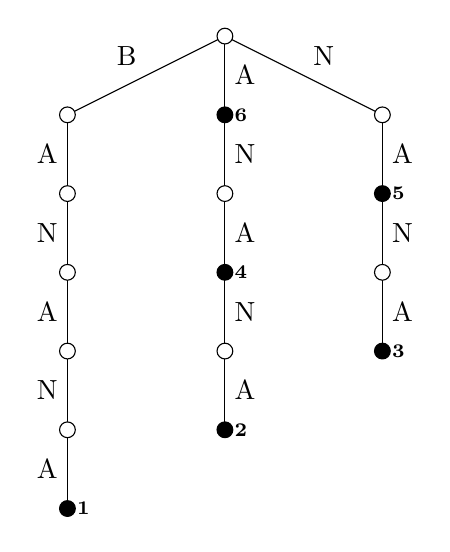
\begin{tikzpicture}
            \coordinate (A) at (4, 7);
            \coordinate (B1) at (2, 6);
            \coordinate (B2) at (4, 6);
            \coordinate (B3) at (6, 6);
            \coordinate (C1) at (2, 5);
            \coordinate (C2) at (4, 5);
            \coordinate (C3) at (6, 5);
            \coordinate (D1) at (2, 4);
            \coordinate (D2) at (4, 4);
            \coordinate (D3) at (6, 4);
            \coordinate (E1) at (2, 3);
            \coordinate (E2) at (4, 3);
            \coordinate (E3) at (6, 3);
            \coordinate (F1) at (2, 2);
            \coordinate (F2) at (4, 2);
            \coordinate (G1) at (2, 1);

            \draw (A) -- node[anchor=south east] { B } (B1);
            \draw (A) -- node[anchor=west] { A } (B2);
            \draw (A) -- node[anchor=south west] { N } (B3);
            \draw (B1) -- node[anchor=east] { A } (C1);
            \draw (B2) -- node[anchor=west] { N } (C2);
            \draw (B3) -- node[anchor=west] { A } (C3);
            \draw (C1) -- node[anchor=east] { N } (D1);
            \draw (C2) -- node[anchor=west] { A } (D2);
            \draw (C3) -- node[anchor=west] { N } (D3);
            \draw (D1) -- node[anchor=east] { A } (E1);
            \draw (D2) -- node[anchor=west] { N } (E2);
            \draw (D3) -- node[anchor=west] { A } (E3);
            \draw (E1) -- node[anchor=east] { N } (F1);
            \draw (E2) -- node[anchor=west] { A } (F2);
            \draw (F1) -- node[anchor=east] { A } (G1);

            \draw[fill=white] (A) circle [radius=.1];

            \draw[fill=white] (B1) circle [radius=.1];
            \draw[fill=black] (B2) circle [radius=.1] node[anchor=west] { \scriptsize \bf 6 };
            \draw[fill=white] (B3) circle [radius=.1];
            \draw[fill=white] (C1) circle [radius=.1];
            \draw[fill=white] (C2) circle [radius=.1];
            \draw[fill=black] (C3) circle [radius=.1] node[anchor=west] { \scriptsize \bf 5 };
            \draw[fill=white] (D1) circle [radius=.1];
            \draw[fill=black] (D2) circle [radius=.1] node[anchor=west] { \scriptsize \bf 4 };
            \draw[fill=white] (D3) circle [radius=.1];
            \draw[fill=white] (E1) circle [radius=.1];
            \draw[fill=white] (E2) circle [radius=.1];
            \draw[fill=black] (E3) circle [radius=.1] node[anchor=west] { \scriptsize \bf 3 };
            \draw[fill=white] (F1) circle [radius=.1];
            \draw[fill=black] (F2) circle [radius=.1] node[anchor=west] { \scriptsize \bf 2 };
            \draw[fill=black] (G1) circle [radius=.1] node[anchor=west] { \scriptsize \bf 1 };


        \end{tikzpicture}
    \end{figure}

\end{frame}
